\section{Evaluatuion and Results} \label{sec:eval}

\begin{figure}
  \begin{center}
    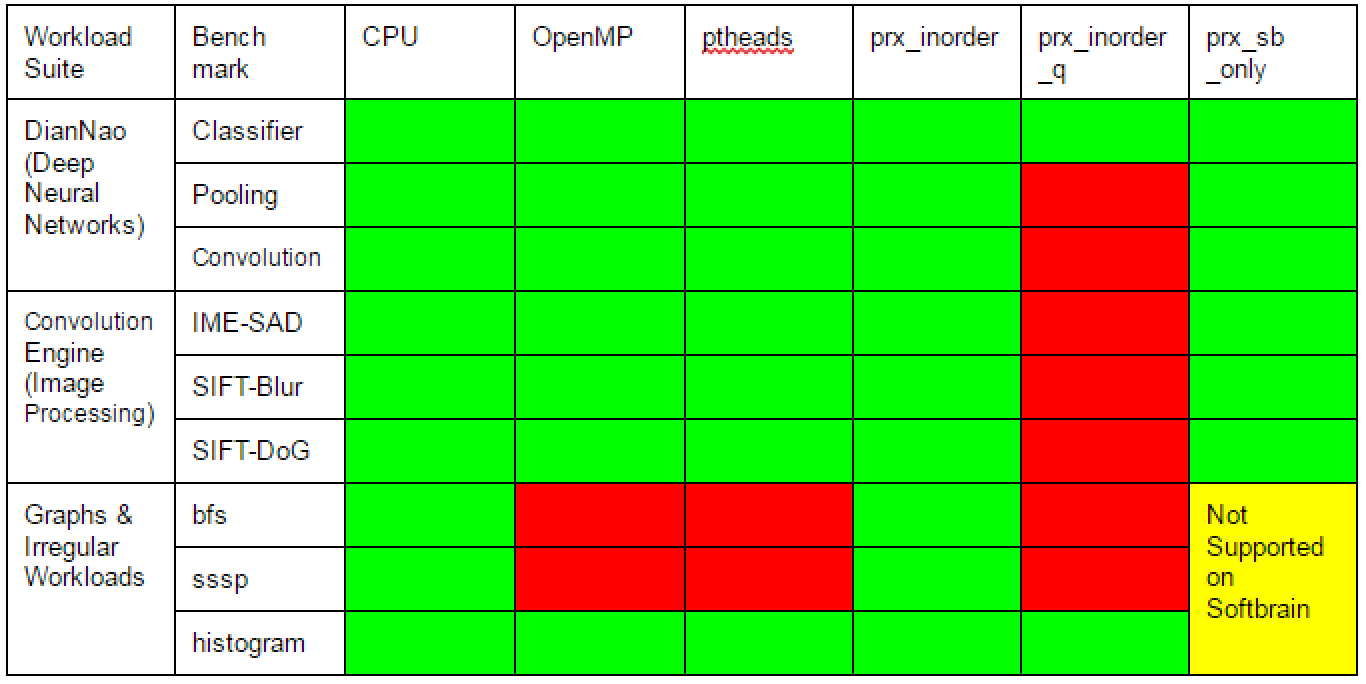
\includegraphics[width=\linewidth]{cs758-figs/workload-progress.png}
  \end{center}
\vspace{-0.2in}
  \caption{Workload progress with respect to their design space. Green means completed and red means future works. Irregular workloads are not supported on softbrain, and is thus colored yellow.}
  \label{fig:workload-progress}
\vspace{-0.05in}
\end{figure}

Figure~\ref{fig:workload-progress} shows the workload progress state for each, and 
show what has been successfuly simulated w.r.t their design space. 


\begin{figure}
  \begin{center}
    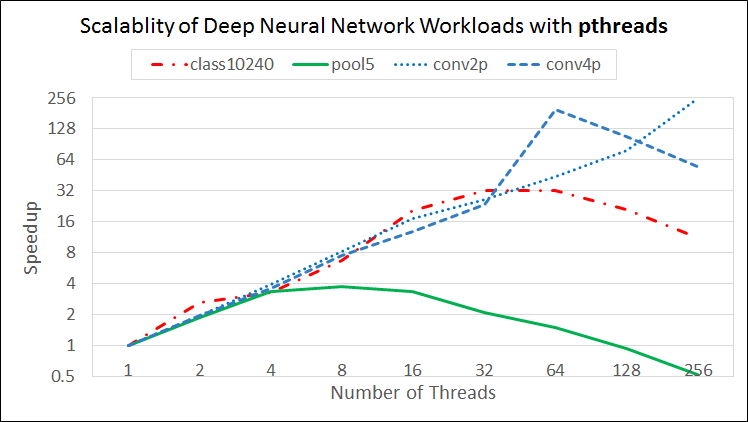
\includegraphics[width=\linewidth]{cs758-figs/scalability-dnn-pthread.png}
  \end{center}
\vspace{-0.2in}
  \caption{Scalability of Deep Neural Network workload suite using pthreads}
  \label{fig:scalability-dnn-pthread}
\vspace{-0.05in}
\end{figure}

Figure~\ref{fig:scalability-dnn-pthread} shows speedups relative to a single 
thread of neural network applications using pthreads on Xeon Phi (godel). 
Classifier (red) exhibits linear speedups up to 32 threads from sharding the 
workload evenly. There is slowdowns after 32 threads due to  shared cache 
capacity, and then slowdown afterwards. Pooling (green) demonstrated poor 
scalability because it aggregates information among a set of neighboring 
inputs, which causes more cache conflicts as the number of threads increases. 
Convolution (blue) is a filtering application, which scales linearly for medium 
sized kernels. However, larger kernels will reach cache capacity bottlenecks and 
demonstrate slowdowns after a certain point. 


\begin{figure}
  \begin{center}
    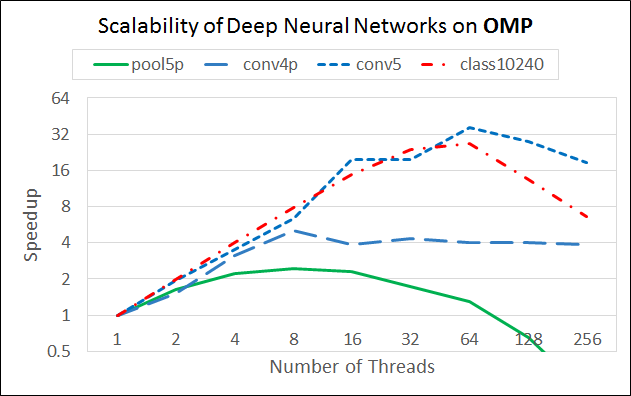
\includegraphics[width=\linewidth]{cs758-figs/scalability-dnn-omp.png}
  \end{center}
\vspace{-0.2in}
  \caption{Scalability of Deep Neural Network workload suite using OpenMP}
  \label{fig:scalability-dnn-omp}
\vspace{-0.05in}
\end{figure}

Figure~\ref{fig:scalability-dnn-omp} shows speedups relative to a single thread 
of neural network applications using OpenMP on Xeon Phi. In general, pthreads 
requires the programmer to do more work and partition data evenly among threads. 
On the other hand, OpenMP is easier to program simply by adding a pragma omp 
parallel. Therefore, pthreads usually requires more work to get better speedups 
and OpenMP requires almost no work to get decent speedups. 


\begin{figure}
  \begin{center}
    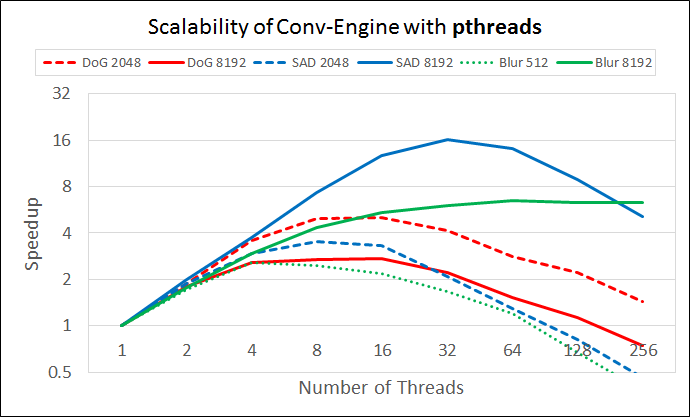
\includegraphics[width=\linewidth]{cs758-figs/scalability-convEngine-pthread.png}
  \end{center}
\vspace{-0.2in}
  \caption{Scalability of Convolution Engine workload suite using pthreads}
  \label{fig:scalability-convEngine-pthread}
\vspace{-0.05in}
\end{figure}

Figure~\ref{fig:scalability-convEngine-pthread} shows speedups relative to a 
single thread of image processing convolution engine applications using pthreads 
on Xeon Phi. DoG (red) exhibits linear speedups up to 4 threads from sharding 
the workload evenly. There is sublinear speedups up to 16 threads, and slowdowns 
afterwards because of false sharing as each thread is trying to write to the DoG 
pyramid/image. SAD (blue) shows sublinear speedups, and peaks at different 
points based on kernel size because larger kernels allows more parallelism. Blur 
(green) mixes neighboring pixels with each other, so increasing the number of 
threads on small kernels are quick to cause cache conflicts and slowdowns. 


\begin{figure}
  \begin{center}
    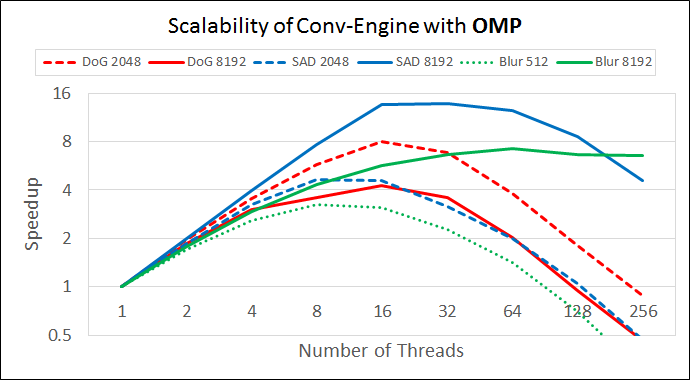
\includegraphics[width=\linewidth]{cs758-figs/scalability-convEngine-omp.png}
  \end{center}
\vspace{-0.2in}
  \caption{Scalability of Convolution Engine workload suite using OpenMP}
  \label{fig:scalability-convEngine-omp}
\vspace{-0.05in}
\end{figure}

Figure~\ref{fig:scalability-convEngine-omp} shows speedups relative to a single 
thread of image processing convolution engine applications using OpenMP on Xeon 
Phi. Note that DoG omp outperforms pthreads, probably because of dynamic 
scheduling. Therefore, comparing proximate to both pthreads and OpenMP is 
important for performance evaluation. 


\begin{figure}
  \begin{center}
    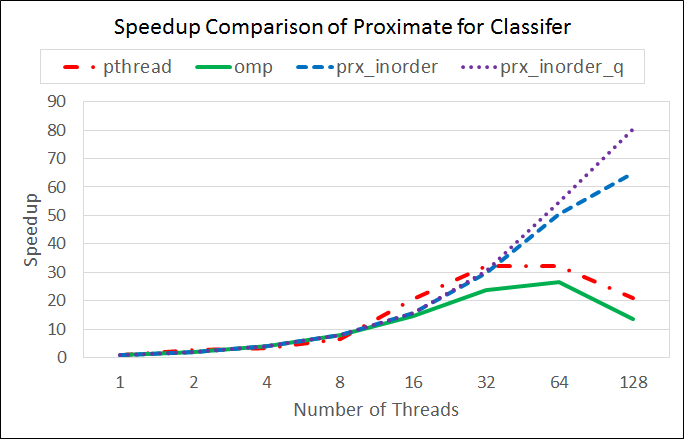
\includegraphics[width=\linewidth]{cs758-figs/speedup-classifier.png}
  \end{center}
\vspace{-0.2in}
  \caption{Speedup comparison of Proximate for Classifier with input size of 10240x10240}
  \label{fig:speedup-classifier}
\vspace{-0.05in}
\end{figure}


Figure~\ref{fig:speedup-classifier} shows speedup analysis of proximate for 
classifier. First we plotted pthreads (red) and omp (green) as baseline speedup 
results on CPU using Xeon Phi. Next, we ran the workload on proximate without 
queuing model, and its’ similarity to pthreads is used to validate the 
simulator. The differences can be attributed to errors in hardware modeling and 
hardware limitation. The preliminary results shows that proximate (with queueing 
model) will given the highest speedup. 

\begin{figure}
  \begin{center}
    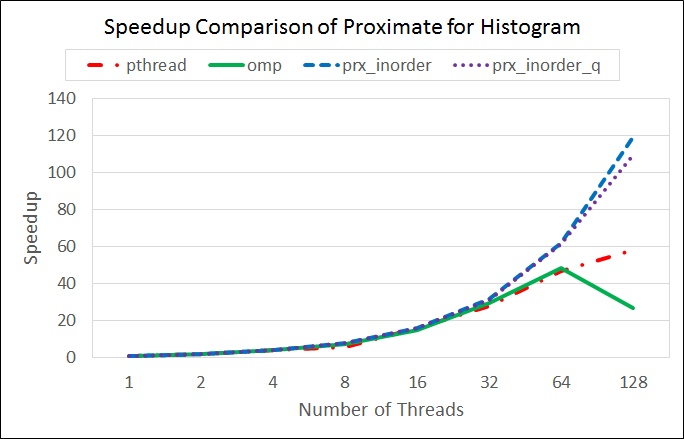
\includegraphics[width=\linewidth]{cs758-figs/speedup-histogram.png}
  \end{center}
\vspace{-0.2in}
  \caption{Speedup comparison of Proximate for Histogram with input size of 470 million pixels}
  \label{fig:speedup-histogram}
\vspace{-0.05in}
\end{figure}

Figure~\ref{fig:speedup-histogram} shows the same speedup analysis of proximate 
for histogram. Although histogram is an irregular workload, 256 values of 3 
colors were small enough to fit in the thread level cache and result in good 
speedups. Proximate again gives the highest performance, which informs us to 
design hardware exactly the way the simulator works to outperform Xeon Phi. 


\begin{figure}
  \begin{center}
    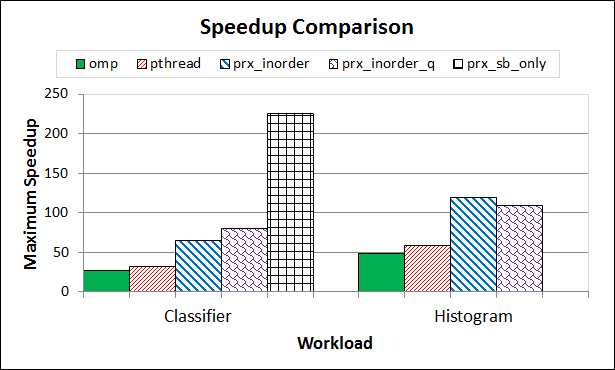
\includegraphics[width=\linewidth]{cs758-figs/speedup-comparison.png}
  \end{center}
\vspace{-0.2in}
  \caption{Speedup comparison between multiple proximate configurations}
  \label{fig:speedup-comparison}
\vspace{-0.05in}
\end{figure}

Figure~\ref{fig:speedup-comparison} shows summarizes how different programming 
paradigms compare on different workloads to compare omp with the optimal number 
of threads on Xeon Phi vs pthreads with optimal number of threads on Xeon Phi vs 
proximate with the optimal number of threads versus a single softbrain instance. 
Softbrain does not support irregular workloads such as histogram. In general, 
proximate is about twice as fast as pthreads, and pthreads is about 20% faster 
than omp. 
